\documentclass[a4paper,spanish]{article}
\usepackage[spanish, activeacute]{babel}
\usepackage{fancyhdr}
\usepackage{ecarat}
\usepackage{graphicx}
\usepackage{amssymb}
\usepackage{listings}
\usepackage[all]{xy} 
\usepackage{clrscode}
\usepackage{moreverb}

\usepackage{verbatimbox}

\oddsidemargin 0in
\textwidth 6.2in
\topmargin 0in
\textheight 18cm
\addtolength{\topmargin}{-.5in}
%textheight 10in
\textheight 24cm
\parskip=1ex
\pagestyle{fancy}
\newcommand{\real}{\hbox{\bf R}}

%  \CodigoF{<Titulo>}{<Archivo>}
\newcommand{\CodigoF}[2]{
  \subsubsection{#1}
  \verbatimtabinput[4]{#2}
}

%\newcommand{\resultadoTP}[1]{
%	\fboxsep 8pt
%	\framebox[15cm][l]{\texttt{#1}}
%	\fboxsep 0pt
%}

%\newcommand{\resultadoTPtexto}[1]{
%	\fboxsep 8pt
%	\framebox[15cm][l]{\texttt{#1}}
%	\fboxsep 0pt
%}

%\newenvironment{fred}
%{\minipage{15cm}\verbatim}
%{\endverbatim\endminipage}

%\newenvironment{last}
%{\verbbox}
%{\endverbbox \fbox{\theverbbox[t]}}

\newcount\entrada
\newcount\base
\newif\ifgarb
\def\imagenHoja{\entrada=\thepage \base=-11
\loop
    \ifnum\entrada<-\base \garbfalse
        \else\garbtrue
        \advance\entrada by \base\fi
    \ifgarb%\number\entrada\\
\repeat
\advance\entrada by 1
    \includegraphics[scale=0.40]{marios/m\number\entrada.png} 
}

\newenvironment{lastTwo}
{\verbbox}
{\endverbbox \rule{\linewidth}{0.1mm}\vspace{6pt}\\\theverbbox\\\rule{\linewidth}{0.1mm}}

\fboxsep 4pt

\begin{document}


\materia{Sistemas Operativos}
\submateria{Segundo Cuatrimestre de 2008}
\titulo{Trabajo pr\'{a}ctico}
\subtitulo{Grupo 8}
\abst{Investigaci'on e implementaci'on de distintas funcionalidades de un
Ubuntu JeOS corriendo sobre una m'aquina virtual (Virtual BOX). Threads,
pipes, fork, join, acceso al kernel mediante m'odulos. Manejo de la consola
y organizaci'on de archivos y carpetas del Sistema Operativo linux.}
\claves{Ubuntu JeOS, M'odulo del kernel, Threads}
\integrante{Mat\'{i}as L\'{o}pez y Rosenfeld}{437/03}{matiaslopez@gmail.com}
\integrante{Rom\'{a}n Gorojovsky}{530/02}{rgorojovsky@gmail.com}
\integrante{Facundo Ciccioli}{399/03}{facundofc@gmail.com}

\thispagestyle{empty}
\maketitle

\lhead{TP Sistemas Operativos}
\rhead{Grupo 8: L\'{o}pez, Gorojovsky, Ciccioli 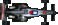
\includegraphics[scale=0.50]{f1.png}}

\cfoot{$\thepage$ de \pageref{fin}}
\lstset{language=C++, numbers=left, tabsize=4}



\tableofcontents
\newpage

%\section{Introducci'on}

	Para la realizaci'on de este trabajo pr'actico nos fue necesario, entre
otras cuestiones log'isticas, aprender a lidiar con las instrucciones de \textit{assembler}.
Esta tarea no nos result'o sencilla en un primer momento, pero gracias a que
mientras hac'iamos tp, tambi'en estudi'abamos para el parcial, fuimos aprendiendo
r'apidamente.

	Uno de los puntos m'as importantes que cabe destacar en la
realizaci'on de este trabajo pr'actico es la gran comodidad que nos permiti'o
para realizarlo la posibilidad de contar con un \textit{svn} para no tener que perder
tiempo intercambi'andonos la 'ultima versi'on y buscando versiones viejas. Esto
nos result'o muy c'omodo ni bien empezamos a programar, cuando de golpe tras
cambiar 3 o 4 l'ineas el programa daba Segmentation Fault (``\textit{Segfaulteaba}'').

	Como metodolog'ia de trabajo no utilizamos ninguna en particular m'as que
ir haciendo las funciones en el orden que figuraban en el enunciado. Esta
``decisi'on'' se ve reflejada en la calidad del c'odigo. Las 'ultimas funciones
aprovechan mucho m'as las operaciones del lenguaje. Desgraciadamente no
contamos con tiempo como para rehacer el trabajo pr'actico, ya que sin duda si
encar'aramos nuevamente las funciones nos saldr'ian distintas. Esto refleja
nuestro aprendizaje a lo largo del desarrollo del tp.

	Salvo las funciones \textbf{checkcolision} y \textbf{salta}, las dem'as
(\textbf{apagar}, \textbf{generarFondo}, \textbf{blit}, \textbf{recortar}) son
funciones que modifican directamente la estructura de un p'ixel. Las 2 primeras
son puramente num'ericas que realizan algunos c'alculos y comparaciones.

	Brevemente podemos describir el funcionamiento de estas 6 funciones as'i
(en orden de realizaci'on):

\begin{itemize}
	\item \textbf{generarFondo}: Pinta el cielo y copia el piso.
	\item \textbf{recortar}: Recorta una parte de un sprite.
	\item \textbf{blit}: Saca el color de off para mimetizar la imagen con el fondo.
	\item \textbf{checkcolision}: Comprueba si hay colisi'on entre 2 objetos, en este
caso, \textbf{Mario} y el ca~no o la caja de las monedas.
	\item \textbf{salta}: Maneja el comportamiento de \textbf{Mario} cuando salta.
	\item \textbf{apagar}: Va cambiando el color de las monedas.
\end{itemize}


%\section{Desarrollo}

\begin{enumerate}
 \item \textsc{generarFondo}:

\item \textsc{Recortar}:

\item \textsc{Blit}:

\item \textsc{checkColision}:

\item \textsc{salta}:

\item \textsc{apagar}:
\end{enumerate}


%\pagebreak
%\section{Resultados}

%\pagebreak
%\section{Discusi'on}

%\section{Conclusiones}


%\newpage
%\section{Algoritmos y c'odigo relevante}\label{imple}
C'odigo de las funciones m'as importantes de nuestra implementaci'on.

\lstset{
	basicstyle=\small,
	showstringspaces=false,
 	language=c,
	keywordstyle=\bfseries,
	stringstyle=\ttfamily,
	tabsize=4
	}

\begin{lstlisting}
typedef struct matriz {
	int filas, columnas;
	double** _matriz;
} Matriz;
\end{lstlisting}


%\newpage
\section{Consignas}

Antes de empezar, ejecute:

\texttt{sudo apt-get install man-db manpages manpages-dev}


De esta manera tendr'a acceso a ayuda en l'inea ejecutando:

\texttt{man <comando>}

Por ejemplo:

\texttt{man cp}

Puede adem'as instalar la versi'on en castellano de la ayuda ejecutando:

\texttt{sudo apt-get install manpages-es}

Para acceder a la ayuda en castellano ejecute por ejemplo:

\texttt{man -L es cp}

Tenga presente que no todos los comandos poseen ayuda en castellano.

\texttt{sudo} permite a usuarios normales ejecutar comandos que requieren permisos de administrador.
Al ejecutar un comando con \texttt{sudo} el sistema le pedir'a su password, y no el password del administrador
(llamado \texttt{root} en Linux, siguiendo la tradici'on de Unix). Esto sucede ya que el sistema permite que
ciertos usuarios (que deber'ian corresponderse con usuarios ``privilegiados'' del sistema) puedan utilizar \texttt{sudo}
ingresando solamente su propio password. El usuario por defecto creado en una instalaci'on de Ubuntu tiene este permiso
y por lo tanto en Ubuntu no es necesario una cuenta de administrador o \texttt{root}.

\texttt{apt-get} es el manejador de paquetes de la distribuci'on Ubuntu. Permite instalar, actualizar y desinstalar
programas. M'as adelante lo utilizaremos para instalar las herramientas necesarias para compilar programas en
Linux.

Si se encontrara detr'as de un proxy, antes de utilizar \texttt{apt-get} debe configurar el proxy. Ejecute el siguiente
comando:

\small
\texttt{sudo echo ''Acquire::http::Proxy $\backslash$''http://proxy.uba.ar:8080$\backslash$'';'' > /etc/apt/apt.conf}
\normalsize

\subsection{Comandos b\'asicos de Unix}

\begin{enumerate}

\item \texttt{pwd} Indique qu'e directorio pasa a ser su directorio actual si ejecuta:

\begin{lastTwo}
/home/mlopez
\end{lastTwo}

\begin{enumerate}
\item \texttt{cd /usr/bin}

\begin{lastTwo}
/usr/bin
\end{lastTwo}

\item \texttt{cd}

\begin{lastTwo}
/home/mlopez
\end{lastTwo}

\item ?`C'omo explica el punto anterior?

\begin{lastTwo}Al utilizar el comando cd sin par'ametros, si existe la variable 
HOME entonces se hace un chdir a ese path.
\end{lastTwo}

\end{enumerate}

\item \texttt{cat} ?`Cu'al es el contenido del archivo \texttt{/home/<usuario>/.profile}?

\begin{lastTwo}
# ~/.profile: executed by the command interpreter for login shells.
# This file is not read by bash(1), if ~/.bash_profile or ~/.bash_login
# exists.
# see /usr/share/doc/bash/examples/startup-files for examples.
# the files are located in the bash-doc package.

# the default umask is set in /etc/profile
#umask 022

# if running bash
if [ -n "$BASH_VERSION" ]; then
    # include .bashrc if it exists
    if [ -f "$HOME/.bashrc" ]; then
	. "$HOME/.bashrc"
    fi
fi

# set PATH so it includes user's private bin if it exists
if [ -d "$HOME/bin" ] ; then
    PATH="$HOME/bin:$PATH"
fi
\end{lastTwo}

\item \texttt{find} Liste \textbf{todos} los archivos que comienzan con \texttt{vmlinuz}.

\begin{lastTwo}
/boot/vmlinuz-2.6.24-19-virtual
/vmlinuz
\end{lastTwo}

Estos archivos son im'agenes del kernel Linux.

\item \texttt{mkdir} Genere un directorio \texttt{/home/<usuario>/tp}.

\begin{lastTwo}
mkdir tp
\end{lastTwo}

\item \texttt{cp} Copie el archivo \texttt{/etc/passwd} al directorio \texttt{/home/<usuario>/tp}.

\begin{lastTwo}
cp /etc/passwd tp/
\end{lastTwo}

\item \texttt{chgrp} Cambie el grupo del archivo \texttt{/home/<usuario>/tp/passwd} para que sea el suyo.

\begin{lastTwo}
El archivo ya es mio, pero en caso de tener que hacerlo: chgrp mlopez passwd.
\end{lastTwo}

\item \texttt{chown} Cambie el due'no del archivo \texttt{/home/<usuario>/tp/passwd} para que sea su usuario.

\begin{lastTwo}
El archivo ya es mio, pero en caso de tener que hacerlo: chown mlopez passwd.
\end{lastTwo}

\item \texttt{chmod} Cambie los permisos del archivo \texttt{/home/<usuario>/tp/passwd} para que:

\begin{lastTwo}
Antes de empezar el pr'oximo paso: chmod 000 passwd para limpiar los permisos originales.
\end{lastTwo}
\begin{itemize}
\item el propietario tenga permisos de lectura, escritura y ejecuci'on

\begin{lastTwo}
chmod u+r+w+x passwd
\end{lastTwo}

\item el grupo tenga s'olo permisos de lectura y ejecuci'on

\begin{lastTwo}
chmod g+r+x passwd
\end{lastTwo}

\item el resto tenga s'olo permisos de ejecuci'on

\begin{lastTwo}
chmod o+x passwd
\end{lastTwo}
\end{itemize}

\item \texttt{grep}

Muestre las l'ineas que tienen el texto ``localhost'' en el archivo \texttt{/etc/hosts}.

\begin{lastTwo}
127.0.0.1	localhost
::1     ip6-localhost ip6-loopback
\end{lastTwo}

Muestre todas las l'ineas que tengan el texto ``POSIX'' de todos los archivos (incluyendo subdirectorios) en \texttt{/etc}.
Evite los archivos binarios y aquellos archivos y directorios que no tienen permiso de lectura para su usuario.

\begin{lastTwo}
grep -R -I -s POSIX /etc/
/etc/init.d/glibc.sh:     echo WARNING: POSIX threads library NPTL requires kernel version
/etc/alternatives/updatedb:\# What shell shoud we use?  We should use a POSIX-ish sh.
/etc/security/limits.conf:\# - msgqueue - max memory used by POSIX message queues (bytes)
\end{lastTwo}

\item \texttt{passwd} Cambie su password.

\begin{lastTwo}
(current) UNIX password:
Enter new UNIX password:
Retype new UNIX password:
passwd: password updated successfully
\end{lastTwo}

\item \texttt{rm} Borre el archivo \texttt{/home/<usuario>/tp/passwd}

\item \texttt{ln}

Enlazar el archivo \texttt{/etc/passwd} a los archivos \texttt{/tmp/contra1} y \texttt{/tmp/contra2}.

Hacer un \texttt{ls -l} para ver cuantos enlaces tiene \texttt{/etc/passwd}.

\begin{lastTwo}
-rw-r--r-- 3 root root 981 2008-10-08 01:11 /etc/passwd
\end{lastTwo}

Estos enlaces se llaman ``hardlinks''. Cada nuevo enlace referencia el mismo espacio ocupado del disco r'igido,
y por lo tanto cada hardlink es igual de representativo de esos bytes ocupados del disco r'igido.
El espacio ocupado solamente se liberar'a cuando todos los enlaces hayan sido borrados.

Ahora enlace el archivo \texttt{/etc/passwd} de manera ``soft'' al archivo \texttt{contra3}.

Verifique con \texttt{ls -l} que no aument'o la cantidad de enlaces de \texttt{/etc/passwd}.

\begin{lastTwo}
mlopez@esparrago:~/tp$ ln -s /etc/passwd /tmp/contra3
mlopez@esparrago:~/tp$ ls -l /etc/passwd
-rw-r--r-- 3 root root 981 2008-10-08 01:11 /etc/passwd
mlopez@esparrago:~/tp$ ls -l /tmp/c*
-rw-r--r-- 3 root   root   981 2008-10-08 01:11 /tmp/contra1
-rw-r--r-- 3 root   root   981 2008-10-08 01:11 /tmp/contra2
lrwxrwxrwx 1 mlopez mlopez  11 2008-11-15 18:38 /tmp/contra3 -> /etc/passwd
\end{lastTwo}

Estos enlaces se llaman ``softlinks'' y apuntan no a los bytes del disco r'igido sino a la ruta del archivo a ser enlazado.
Operar sobre el softlink es igual que operar sobre el archivo, sin embargo los softlinks no cuentan en la cantidad de
enlaces (ya que no apuntan a los bytes ocupados del disco r'igido) y pueden ser borrados sin afectar al archivo original,
aunque si se borra el archivo original el softlink quedar'a hu'erfano y no apuntar'a a nada.

\item \texttt{mount}

Monte el CD-ROM de instalaci'on de Ubuntu JeOS y liste su contenido.

Para hacer esto deber'a especificar la ISO de instalaci'on de Ubuntu JeOS como CD-ROM de la m'aquina virtual.
Si bien puede hacer esto como lo hizo para instalar el sistema, si la m'aquina virtual est'a corriendo debe hacer click
derecho en el 'icono con forma de CD-ROM en la esquina inferior derecha de la m'aquina virtual, y seleccionar
\textbf{CD/DVD-ROM Image...} (ver figura \ref{isocdrom3}). En la ventana que aparece seleccione la ISO de instalaci'on
(ver figura \ref{isocdrom4}).

%\Imagen{vb_ubuntu/vb_isocdrom3.png}{7cm}{Usando una imagen ISO con la m'aquina virtual corriendo.}{isocdrom3}
%\Imagen{vb_ubuntu/vb_isocdrom4.png}{7cm}{Seleccionando la ISO de instalaci'on.}{isocdrom4}

Presente los filesystems que tiene montados.

\begin{lastTwo}
mlopez@esparrago:~/tp$ sudo mount /dev/cdrom /media/cdrom
mount: block device /dev/scd0 is write-protected, mounting read-only
mlopez@esparrago:~/tp$ mount
/dev/sda1 on / type ext3 (rw,relatime,errors=remount-ro)
proc on /proc type proc (rw,noexec,nosuid,nodev)
/sys on /sys type sysfs (rw,noexec,nosuid,nodev)
varrun on /var/run type tmpfs (rw,noexec,nosuid,nodev,mode=0755)
varlock on /var/lock type tmpfs (rw,noexec,nosuid,nodev,mode=1777)
udev on /dev type tmpfs (rw,mode=0755)
devshm on /dev/shm type tmpfs (rw)
devpts on /dev/pts type devpts (rw,gid=5,mode=620)
share on comp/ type vboxsf (uid=1000,gid=1000,rw)
\end{lastTwo}

\item \texttt{df} ?`Qu'e espacio libre tiene cada uno de los filesystems montados?

\begin{lastTwo}
mlopez@esparrago:~/tp$ df -h
Filesystem            Size  Used Avail Use% Mounted on
/dev/sda1             494M  427M   42M  92% /
varrun                 62M   32K   62M   1% /var/run
varlock                62M     0   62M   0% /var/lock
udev                   62M   40K   62M   1% /dev
devshm                 62M     0   62M   0% /dev/shm
df: `comp/': No such file or directory
/dev/scd0             100M  100M     0 100% /media/cdrom0

comp es una carpeta compartidad con la otra m'aquina
\end{lastTwo}

\item \texttt{ps} ?`Cu'antos procesos de usuario tiene ejecutando? Indique cu'antos son del sistema.

\begin{lastTwo}
ps
  PID TTY          TIME CMD
 3946 tty1     00:00:00 bash
 5528 tty1     00:00:07 vi
 5747 tty1     00:00:00 bash
 5748 tty1     00:00:00 ps
\end{lastTwo}

\begin{lastTwo}
ps aux

USER       PID %CPU %MEM    VSZ   RSS TTY      STAT START   TIME COMMAND
root         1  0.0  1.3   2844  1692 ?        Ss   12:03   0:02 /sbin/init
root         2  0.0  0.0      0     0 ?        S<   12:03   0:00 [kthreadd]
root         3  0.0  0.0      0     0 ?        S<   12:03   0:00 [migration/0]
root         4  0.0  0.0      0     0 ?        S<   12:03   0:00 [ksoftirqd/0]
root         5  0.0  0.0      0     0 ?        S<   12:03   0:00 [watchdog/0]
root         6  0.0  0.0      0     0 ?        S<   12:03   0:10 [events/0]
root         7  0.0  0.0      0     0 ?        S<   12:03   0:00 [khelper]
root        36  0.0  0.0      0     0 ?        S<   12:03   0:00 [kblockd/0]
root        39  0.0  0.0      0     0 ?        S<   12:03   0:00 [kacpid]
root        40  0.0  0.0      0     0 ?        S<   12:03   0:00 [kacpi_notify]
root        80  0.0  0.0      0     0 ?        S<   12:03   0:00 [kseriod]
root       115  0.0  0.0      0     0 ?        S    12:03   0:00 [pdflush]
root       116  0.0  0.0      0     0 ?        S    12:03   0:00 [pdflush]
root       117  0.0  0.0      0     0 ?        S<   12:03   0:00 [kswapd0]
root       160  0.0  0.0      0     0 ?        S<   12:03   0:00 [aio/0]
root      1216  0.0  0.0      0     0 ?        S<   12:03   0:00 [ata/0]
root      1219  0.0  0.0      0     0 ?        S<   12:03   0:00 [ata_aux]
root      1239  0.0  0.0      0     0 ?        S<   12:03   0:00 [scsi_eh_0]
root      1241  0.0  0.0      0     0 ?        S<   12:03   0:00 [scsi_eh_1]
root      2207  0.0  0.0      0     0 ?        S<   12:03   0:00 [kjournald]
root      2346  0.0  0.5   2220   668 ?        S<s  12:03   0:03 /sbin/udevd --daemon
root      2536  0.0  0.0      0     0 ?        S<   12:03   0:00 [kpsmoused]
dhcp      3484  0.0  0.4   2436   548 ?        S<s  12:04   0:00 dhclient3 -e IF_METRIC=100 -pf /var/run/dhclient.eth0.pid -lf /var/lib/dhcp3/dhclient.eth0.leases eth0
root      3813  0.0  0.4   1716   508 tty4     Ss+  12:04   0:00 /sbin/getty 38400 tty4
root      3816  0.0  0.4   1716   508 tty5     Ss+  12:04   0:00 /sbin/getty 38400 tty5
root      3820  0.0  0.9   2568  1208 tty2     Ss   12:04   0:00 /bin/login --       
root      3824  0.0  0.4   1716   508 tty3     Ss+  12:04   0:00 /sbin/getty 38400 tty3
root      3826  0.0  0.4   1716   504 tty6     Ss+  12:04   0:00 /sbin/getty 38400 tty6
root      3847  0.0  0.1   1844   236 ?        Ss   12:04   0:00 /usr/sbin/vboxadd-timesync --daemonize
syslog    3890  0.0  0.5   1936   648 ?        Ss   12:04   0:00 /sbin/syslogd -u syslog
root      3909  0.0  0.4   1868   532 ?        S    12:04   0:00 /bin/dd bs 1 if /proc/kmsg of /var/run/klogd/kmsg
klog      3911  0.0  1.4   2896  1784 ?        Ss   12:04   0:00 /sbin/klogd -P /var/run/klogd/kmsg
root      3926  0.0  0.3   1764   396 ?        Ss   12:04   0:01 /usr/sbin/gpm -m /dev/input/mice -t exps2
root      3945  0.0  0.9   2568  1204 tty1     Ss   12:04   0:00 /bin/login --       
mlopez    3946  0.0  1.8   4804  2280 tty1     S    12:04   0:00 -bash
mlopez    3958  0.0  1.7   4788  2228 tty2     S+   12:17   0:01 -bash
mlopez    5528  0.2  2.6   7060  3304 tty1     S+   17:50   0:08 vi svn/informe/consignas.tex svn/informe/tp1.tex
mlopez    5802  0.0  0.9   3756  1152 tty1     S+   18:53   0:00 /bin/bash -c (ps -aux) >/tmp/v784235/10 2>&1
mlopez    5803  0.0  0.7   2644  1004 tty1     R+   18:53   0:00 ps -aux
\end{lastTwo}

\item \texttt{umount} Desmonte el CD-ROM de instalaci'on de Ubuntu JeOS.

\begin{lastTwo}
sudo umount /media/cdrom
\end{lastTwo}

\item \texttt{uptime} ?`Cuanto tiempo lleva ejecutando su m'aquina virtual?

\begin{lastTwo}
18:48:33 up  6:45,  2 users,  load average: 0.00, 0.00, 0.00
\end{lastTwo}

\item \texttt{uname} ?`Qu'e versi'on del kernel de Linux est'a utilizando?

\begin{lastTwo}
uname -a:  Linux esparrago 2.6.24-19-virtual \#1 SMP Wed Jun 18 15:52:10 UTC 
2008 i686 GNU/Linux
\end{lastTwo}

\end{enumerate}

\subsection{Salida est\'andar y pipes}

\begin{enumerate}

\item STDOUT

\begin{enumerate}

\item Conserve en el archivo \texttt{/home/<usuario>/tp/config} la salida del comando \texttt{ls} que muestra todos los
archivos del directorio \texttt{/etc} y de los subdirectorios bajo \texttt{/etc}.

\begin{lastTwo}
ls -R /etc/ > /home/mlopez/tp/config
\end{lastTwo}

\item Presente cuantas l'ineas, palabras y caracteres tiene \texttt{/home/<usuario>/tp/config}.

\fboxsep 0pt
\begin{lastTwo}
mlopez@esparrago:~/tp$ wc -l config
730 config
mlopez@esparrago:~/tp$ wc -w config
654 config
mlopez@esparrago:~/tp$ wc -m config
8422 config
\end{lastTwo}

\item Agregue el contenido, ordenado alfab'eticamente, del archivo \texttt{/etc/passwd} al final del
archivo \texttt{/home/<usuario>/tp/config}.

\begin{lastTwo}
sort /etc/passwd >> /home/mlopez/tp/config
\end{lastTwo}

\item Presente cuantas l'ineas, palabras y caracteres tiene \texttt{/home/<usuario>/tp/config}.

\begin{lastTwo}
mlopez@esparrago:~/tp$ wc -l config
754 config
mlopez@esparrago:~/tp$ wc -w config
684 config
mlopez@esparrago:~/tp$ wc -m config
9403 config
\end{lastTwo}

\end{enumerate}

\item Pipes

\begin{enumerate}

\item Liste en forma amplia los archivos del directorio \texttt{/usr/bin} que comiencen con la letra ``a''.
Del resultado obtenido, seleccione las l'ineas que contienen el texto \texttt{apt} e informe la cantidad de caracteres,
palabras y l'ineas.

Est'a prohibido, en este 'item, usar archivos temporales de trabajo.

\begin{lastTwo}
mlopez@esparrago:~/tp$ ls -lh /usr/bin/a* | grep apt
-rwxr-xr-x 1 root root  63K 2008-04-22 12:21 /usr/bin/apt-cache
-rwxr-xr-x 1 root root  18K 2008-04-22 12:21 /usr/bin/apt-cdrom
-rwxr-xr-x 1 root root 9.9K 2008-04-22 12:21 /usr/bin/apt-config
-rwxr-xr-x 1 root root  22K 2008-04-22 12:21 /usr/bin/apt-extracttemplates
-rwxr-xr-x 1 root root 187K 2008-04-22 12:21 /usr/bin/apt-ftparchive
-rwxr-xr-x 1 root root 139K 2008-04-22 12:21 /usr/bin/apt-get
-rwxr-xr-x 1 root root 2.2M 2008-04-04 06:56 /usr/bin/aptitude
-rwxr-xr-x 1 root root 1.9K 2008-04-04 06:56 /usr/bin/aptitude-create-state-bundle
-rwxr-xr-x 1 root root 3.0K 2008-04-04 06:56 /usr/bin/aptitude-run-state-bundle
-rwxr-xr-x 1 root root 5.0K 2008-04-22 12:20 /usr/bin/apt-key
-rwxr-xr-x 1 root root 2.2K 2008-04-22 12:20 /usr/bin/apt-mark
-rwxr-xr-x 1 root root  26K 2008-04-22 12:21 /usr/bin/apt-sortpkgs
mlopez@esparrago:~/tp$ ls -lh /usr/bin/a* | grep apt | wc -l
12
mlopez@esparrago:~/tp$ ls -lh /usr/bin/a* | grep apt | wc -w
96
mlopez@esparrago:~/tp$ ls -lh /usr/bin/a* | grep apt | wc -m
817
\end{lastTwo}

\end{enumerate}

\end{enumerate}

\subsection{Scripting}

Escriba un script de shell que sincronice dos carpetas. El script debe recibir las dos carpetas (origen y destino, en ese
orden) desde la l'inea de comando, o preguntarlas interactivamente al usuario en caso de no recibirlas. Adem'as, debe
aceptar un modificador \texttt{-r} que indica modo de operaci'on recursivo.

Una vez conocidas las dos carpetas con las que se operar'a, el script deber'a copiar todos los archivos de la carpeta origen
que no est'en presentes en la carpeta destino, y adem'as tambi'en deber'a copiar todos los archivos presentes en ambas
carpetas que tengan una fecha de modificaci'on posterior en la carpeta origen que en la carpeta destino. De esta manera, al
ejecutar el script, estar'a seguro de que la carpeta destino contiene toda la informaci'on de la carpeta origen, excepto lo
que fue modificado posteriormente en la carpeta destino.

El modificador \texttt{-r} indica al script realizar la sincronizaci'on tambi'en con los archivos de todos los
subdirectorios de la carpetas origen y destino.

\CodigoF{Script de sincronizaci'on}{../grupo8/scriptSincro.sh}

\paragraph{Sugerencia}

Recuerde que generalmente el esp'iritu de los scripts es proveer la m'inima l'ogica necesaria alrededor de otros programas
ya presentes en el sistema que puedan proveer parte de la funcionalidad requerida para resolver un determinado problema.

\subsection{Ejecuci\'on de procesos en background}

Antes de resolver esta secci'on instale los siguientes paquetes en la m'aquina virtual:

\begin{itemize}
\item \texttt{nano}: editor de texto.
\item \texttt{mc}: manejador de archivos.
\item \texttt{gcc}: compilador de C.
\item \texttt{libc6-dev}: biblioteca est'andar de C.
\end{itemize}

Cree el archivo \texttt{/home/<usuario>/tp/loop.c}. Comp'ilelo con \texttt{gcc}. El programa compilado debe llamarse
\texttt{loop}.

\begin{lastTwo}
gcc -o loop loop.c
\end{lastTwo}

\CodigoF{loop.c}{../grupo8/loop.c}

\begin{enumerate}
\item Correrlo en foreground. ?`Qu'e sucede? Mate el proceso con \texttt{Ctrl-c}.

\begin{lastTwo}
Imprime consecutivamente los n'umeros del 48 al 55.
\end{lastTwo}

\item Ahora ejec'utelo en background: \texttt{/usr/src/loop > /dev/null \&}. Mate el proceso con el comando \texttt{kill}.

\begin{lastTwo}
mlopez@esparrago:~/tp$ /home/mlopez/tp/loop > /dev/null &
[1] 3880
mlopez@esparrago:~/tp$ ps
  PID TTY          TIME CMD
 3848 tty2     00:00:00 bash
 3880 tty2     00:00:09 loop
 3881 tty2     00:00:00 ps
mlopez@esparrago:~/tp$ kill -9 3880
mlopez@esparrago:~/tp$ ps
  PID TTY          TIME CMD
 3848 tty2     00:00:00 bash
 3882 tty2     00:00:00 ps
[1]+  Killed                  /home/mlopez/tp/loop > /dev/null
\end{lastTwo}

\end{enumerate}

\subsection{IPC y sincronizaci\'on}

\subsubsection{Pipes}

Muestre con un ejemplo en lenguaje C como realizar exclusi'on mutua entre dos procesos utilizando un s'olo pipe.

\paragraph{Sugerencia}

Revise la ayuda de la llamada al sistema \texttt{pipe} para construir el pipe y de \texttt{fork} para crear
nuevos procesos.

\CodigoF{pipe.c}{../grupo8/pipe.c}

\subsubsection{Threads}

Antes de resolver este ejercicio instale el paquete \texttt{glibc-doc}.

Resuelva el problema de productor/consumidor utilizando threads.

\paragraph{Sugerencia}

Revise la ayuda de \texttt{pthreads}, la implementaci'on de threads en Linux, para conocer los mecanismos de creaci'on y
destrucci'on de threads. Adem'as, \texttt{pthreads} provee mecanismos de sincronizaci'on que le ayudar'an a resolver este
ejercicio.


\CodigoF{productorConsumidor.c}{../grupo8/productorConsumidor.c}

\subsection{El kernel Linux}

Antes de resolver esta secci'on instale los siguientes paquetes en la m'aquina virtual:

\begin{itemize}
\item \texttt{make}: utilidad para mantener grupos de programas.
\item \texttt{linux-headers-<version>}: headers del kernel de Linux.
\end{itemize}

Sustituya \texttt{<version>} por el resultado del comando \texttt{uname -r}.

\subsubsection{Funcionamiento del kernel Linux}

\begin{enumerate}

\item Describa la administraci'on del procesador utilizada por defecto en el kernel Linux.

\subitem {\tt
La administraci\'on del procesador de Linux utiliza el m\'etodo de round robin. Este sistema permite que varios procesos puedan estar ejecutandose al mismo tiempo (hablando en sentido de procesos concurrentes, a menos de que se cuente con 2 procesadores, nunca se va a poder tener 2 procesos ejecutandose a la vez), lo que quiere decir que la CPU esta dividida en ``partes'', cada uno para un proceso particular. Si uno de ellos no termina para cuando su porci\'on de tiempo (quantum) expira, un intercambio de procesos puede ocurrir (en caso de que haya alguno en cola de espera). Esta administraci\'on utiliza interrupciones por tiempo  que se generean cada vez que el quantum transcurri'o. Debido a todo esto, no es necesario c\'odigo adicional dentro de los procesos para que la CPU pueda mantenerlos corriendo concurrementemente.

La pol\'itica de administraci\'on se basa en enumerar procesos de acuerdo a su prioridad dentro del sistema. Hay algor\'itmos complicados para definir el orden en el cual los procesos deben ser ejecutados para optimizar el rendimiento, pero siempre se mantiene el hecho de que a cada proceso se le asigna un n\'umero que corrresponde a que tan apropiado es de ser asignado a la CPU.

La asignaci\'on de prioridades es din'amica dentro de Linux. Cuando a un proceso se le nego por mucho tiempo el uso de la CPU, se le incrementa su prioridad. Lo mismo pasa si un proceso se ejecuta por demasiado tiempo, como penalidad se le decrementa su prioridad. Gracias a esto se evita que un proceso se mantenga inactivo por mucho tiempo o que consuma demasiado los ciclos del procesador.
}

\item Describa la administraci'on de memoria utilizada por defecto en el kernel Linux.

\subitem {\tt Cuando el procesador ejecuta un programa, esta leyendo una instrucci\'on desde la memoria y la decodifica. Por lo general, esa instrucci\'on necesita alguno datos, por lo que el procesador deber'a realizar un nuevo acceso a memoria para poder darselos al proceso mismo. De esta manera, el procesador esta siempre accediendo a memoria para traer datos o instrucciones. Utilizando memoria virtual, todas las direcciones a las cuales el procesador accede no son f\'isicas, las cuales permiten que, junto con un set de tablas dentro del sistema operativo, se pueda convertir estas direcciones virtuales en direcciones reales. 

Como hay menos memoria f\'isica que la memoria virtual, el sistema debe  tener mucho cuidado en no usar la memoria f\'isica ineficientemente. Cuando un proceso intenta acceder a una direcci\'on virtual que no se encuentra dentro de las asignadas a \'el, el procesador no puede encontrar una tabla de pagina cuya entrada sea la direccion pedida. Esto quiere decir que el proceso esta pidiendo una direcci\'on que no le corresponde, por lo que el sistema lo terminar'a (al proceso). 

Linux usa paginaci\'on por demanda como sistema de administraci\'on de memoria. Carga imagenes ejecutables a la memoria virtual de un proceso para su utilizaci'on. Cada vez que un comando se ejecuta, el archivo que lo contiene es abierto y sus contenidos son mapeados a la memoria virtual del proceso. Esto se conoce con el nombre de mapeo de memoria. Cuando el proceso se ejecuta, s'olo una parte de este esta en memoria f\'isica, el resto esta dentro del disco (el dispositivo que se utiliza como memoria virtual), por lo que el sistema usara el mapa de memoria para ir dandole al proceso toda la informaci\'on necesaria para su ejecuci\'on. Si un proceso necesita volcar una p\'agina virtual dentro de la memoria f\'isica, y no hay suficiente espacio en ella, el sistema debe conseguir lugar para esta p\'agina, descartando cualquier otra de la misma. A veces, la p\'agina que se va a descartar no sufri\'o cambio alguno, por lo que no debe ser guardada. Sin embargo, si la p\'agina fue modificada, el sistema debe preservar los contenidos de esa p\'agina para que pueda ser leida mas tarde. Este tipo de p\'agina que fue modificada se guarda dentro de un archivo conocido como "swap file". Linux utiliza LRU (Least Recently Used) para definir que p\'agina ser'a quitada para poner otra nueva. Mientras m'as sea utilizada una determinada p\'agina, tendr\'a menos posibilidades de ser swapeada que una p\'agina que se utiliza menos.
}

\item Describa el sistema de archivos utilizado en la distribuci'on de Linux que instal'o en la m'aquina virtual.
?`Qu'e capas existen en el kernel Linux para soportar sistemas de archivos sobre dispositivos de bloques?

\subitem {\tt Dentro de los sistemas Linux, se cuenta con un sistema de archivos virtual, que es el encargado de manejar los filesystems dentro del sistema. \'Este se conoce mas por sus siglas en ingles: VFS (Virtual File System). El concepto es poder separar los filesystems de bajo nivel con el resto del Kernel, para as\'i no tener que repensar el Kernel para querer cambiar el sistema de archivos sobre el cual esta montado. De esta manera, ser\'a posible un manejo de los archivos eficaz sin importar el sistema que se utilize. Es decir, Linux puede utilizar cualquier filesystem (ext2, ext3, fat, vfat, ufs, etc) gracias a el uso del VFS. El VFS brinda el set de instrucciones necesario y generales para todos los filesystems para poder usarlos a gusto del sistema (o del programador). Las estructuras atrav\'ez de las cuales el VFS funciona son: los index-nodes, que son atravez de los cuales se mantiene un registro de los file; una cach\'e de directorios para acelerar la b\'usqueda y mapeado de nombres de ficheros con sus correspondientes inodos y el super bloque, que es donde se carga cada filesystem para poder ser usado.

La distribucion instalada dentro de este trabajo practico contiene a ext3 como su filesystem. Ext3 (third extended filesystem o "tercer sistema de archivos extendido") es un sistema de archivos con registro por diario (journaling). Este concepto se basa en llevar un journal o registro de diario en el que se almacena la informaci\'on necesaria para restablecer los datos afectados por la transacci\'on en caso de que \'esta falle.}

\end{enumerate}

\subsubsection{M'odulos de kernel}

El kernel de Linux permite ser ampliado en \textbf{runtime} con m'odulos. Los m'odulos son objetos de c'odigo compilado
que pueden ser insertados en runtime al kernel, siendo linkeados contra el kernel al momento de ser insertados. De esta
manera puede ampliarser la funcionalidad del kernel en runtime, sin tener que incluir todo el c'odigo en el binario
original.

\subsubsection{Compilando un m'odulo de kernel}

En esta secci'on omitimos el enunciado y vamos directo a lo que hicimos.

\CodigoF{cambiarLuces.c}{../grupo8/cambiarLuces.c}

Para compilar este c'odigo deber'a construir una \textbf{Makefile}. Este archivo Makefile es utilizado luego por el
comando \texttt{make} para compilar el m'odulo con las opciones correctas. En el mismo directorio donde se encuentra
\texttt{cambiarLuces.c} cree un archivo \texttt{Makefile} conteniendo:

\CodigoF{Makefile}{../grupo8/Makefile.txt}

Luego ejecute:

\texttt{make}

Para compilar el m'odulo. Finalmente, pruebe insertar el m'odulo usando:

\texttt{insmod cambiarLuces.ko} esto tambi'en viene facilitado con el siguiente script
\CodigoF{./cargarKernel.sh}{../grupo8/cargarKernel.sh}

Deber'ia ver un mensaje en la consola indicando que se cargo correctamente o que fall'o. 

Para hacer funcionar el m'odulo escribir como root en \texttt{/proc/lasluces/escribaAqui} o, nuevamente, con un script que toma un dato:

\CodigoF{./escribir.sh dato}{../grupo8/escribir.sh}

Para sacar el m'odulo:

\texttt{rmmod cambiarLuces.ko} o su versi'on script.

\CodigoF{./descargarKernel.sh }{../grupo8/descargarKernel.sh}

Esto tambi'en deber'ia dar un mensaje indicando lo sucedido.

\subsubsection{Un m'odulo propio}

Escriba un m'odulo de kernel que permita controlar los LEDs del teclado \textbf{sin necesidad de escribir un programa 
en lenguaje C}. El m'odulo deber'a permitir prender o apagar cada LED usando simplemente comandos del shell.

Dado que la m'aquina virtual provista por VirtualBox no muestra el estado de los LEDs, la c'atedra provee abajo
un programa que lo hace. Compile utilizando:

\texttt{gcc -o check\_kbleds check\_kbleds.c}

\CodigoF{check\_kbleds.c}{../grupo8/checkkbleds.c}

\paragraph{Sugerencia}

Haga que su m'odulo cree un archivo en \texttt{/proc} y que las escrituras a ese archivo controlen los LEDs utilizando 
la IOCTL \texttt{KDSETLED} de la consola de Linux.


\appendix
%\newpage
%
\begin{centering}
\bf Laboratorio de M\'etodos Num\'ericos - Primer Cuatrimestre 2007 \\
\bf Trabajo Pr\'actico N\'umero 4: Luigi s\'olo admira a las Ferraris \\
\end{centering}

\vskip 1 cm
\hrule
\vskip 0.5 cm

\textbf{Introducci\'on}

Nos encontramos en el grupo de an\'alisis num\'erico de uno de los equipos de
F\'ormula 1, y estamos a pocas semanas de un gran premio que se realizar\'a
en un aut\'odromo a\'un no visitado por la categor\'\i a. Nos enfrentamos
al serio problema de decidir la mejor forma de tomar las curvas del nuevo
circuito, y para esto solamente podemos realizar simulaciones, dado que
el fin de semana de la carrera ser\'a la primera vez que nuestros autos
tomen contacto con esta pista.

Consideremos una curva del circuito, como la que muestra la Figura 1.
Queremos que nuestro auto comience en alg\'un punto del segmento A con
una cierta velocidad inicial, y que llegue a alg\'un punto del segmento B en
buenas condiciones (es decir, a una buena velocidad final, con las cuatro
ruedas sobre el pavimento y con la carrocer\'\i a en su lugar). Nuestro
objetivo principal es que el auto pueda sortear la curva sin derrapar, dado
que a la velocidad a la que circula se pierde el control muy r\'apidamente
si el auto pierde adherencia.

\vskip 11pt

\begin{centering}
\includegraphics{tp4-1.png} \\
Figura 1: Ejemplo de una curva y los puntos que determinan la trayectoria. \\
\end{centering}

\vskip 11pt

Para esto, trazamos una serie de puntos por los que esperamos que pase
el auto a intervalos regulares de $\omega = 0.1$ sg. Es decir, en el
instante $t=0$ sg.~el auto estar\'a en $p_1$, en el instante
$t=0.1$ sg.~estar\'a en $p_2$, etc. Como los puntos corresponden a
instantes equiespaciados en el tiempo, entonces estar\'an m\'as separados
en los tramos en los que el auto circule a mayor velocidad, y estar\'an
m\'as juntos en los tramos en los que el auto disminuya su velocidad.

Para determinar la trayectoria
completa del auto, utilizamos un spline param\'etrico que interpole estos
puntos, con lo cual tendremos una funci\'on $T:\real\to\real^2$ que nos
indicar\'a expl\'\i citamente la posici\'on del auto en funci\'on del tiempo.
Es decir, en el instante $t$, el auto se encuentra en el punto $T(t)$. Notar
que en funci\'on de este spline tambi\'en podemos calcular el vector velocidad y
el vector aceleraci\'on en cada instante de la trayectoria.

\vfil \eject

\textbf{C\'omo decidir si el auto se sale de la trayectoria}

Sea $t$ un instante del recorrido, en el cual el auto se encuentra en el
punto $T(t)\in\real^2$. Llamemos $v(t)$ y $a(t)$ al m\'odulo del
vector velocidad y al m\'odulo del vector aceleraci\'on en el instante $t$,
respectivamente. En este instante, la fuerza de frenado que ejerce el auto
sobre el piso es $F(t) = m\: a(t)$, siendo $m$ la masa del auto. El auto
no patina en el instante $t$ si
\begin{equation}
F(t) \ \le\ (mg + v(t)^2s) \: \mu_0. \label{condicion}
\end{equation}
En esta f\'ormula, $g=9.81$ m/sg${}^2$ es la aceleraci\'on gravitatoria,
$s$ es el coeficiente de carga din\'amica (de modo tal que $v(t)^2 s\mu_0$ es
la fuerza que ejerce el aire sobre la superficie del veh\'\i culo en
direcci\'on normal a la superficie de la pista, representando la acci\'on
de los alerones), y $\mu_0$ es el coeficiente de rozamiento est\'atico
(que depende del compuesto de los neum\'aticos, de la composici\'on del
pavimento y de las temperaturas del piso y de los neum\'aticos). El auto
se mantiene dentro de la trayectoria sin derrapar si la condici\'on
(\ref{condicion}) se cumple en todos los puntos de la misma.

\textbf{Enunciado}

El objetivo del trabajo pr\'actico es implementar un programa que tome los
datos del auto y de la trayectoria desde un archivo, que calcule un
spline param\'etrico que interpole los puntos de la trayectoria y que
determine si en alg\'un punto del recorrido el auto pierde adherencia. En
caso positivo, el programa deber\'a informar el punto en el cual esto
sucede, y la velocidad y direcci\'on del auto en ese momento.

El programa deber\'a tomar los datos de entrada desde un archivo de texto
cuyo formato queda a criterio del grupo. Debe notarse que los datos de
entrada incluyen, adem\'as de los puntos de la trayectoria, los datos del
auto (masa, coeficiente de rozamiento, coeficiente de carga din\'amica, etc.)
y el intervalo $\omega$ entre puntos consecutivos de la trayectoria.

Se deber\'a utilizar un algoritmo eficiente para el c\'alculo del spline
param\'etrico. Se debe mencionar en el informe el tipo de spline que se usa
para la interpolaci\'on, comentando las diferentes opciones consideradas
y las razones que llevaron a seleccionar esta opci\'on.

El c\'alculo para determinar si el auto derrapa en alg\'un punto de la
trayectoria deber\'a estar basado en un m\'etodo num\'erico a elecci\'on del
grupo para buscar m\'aximos o m\'\i nimos de funciones de una variable.
Sugerimos consultar con los docentes antes de utilizar alg\'un m\'etodo
num\'erico que no se encuentre dentro de esta categor\'\i a.

Adem\'as de estos puntos obligatorios, los invitamos a implementar los
siguientes \'\i tems optativos que pueden ser de inter\'es para el
an\'alisis:
\begin{itemize}
\item Realizar gr\'aficos de la velocidad y la aceleraci\'on en funci\'on
del tiempo. Tambi\'en puede ser interesante graficar la fuerza $F(t)$ en
funci\'on del tiempo, para ver en qu\'e momento el giro se torna peligroso.
\item Mostrar una animaci\'on en pantalla de la trayectoria del auto, junto
con su vector velocidad y la fuerza de frenado, para ver c\'omo evolucionan
a medida que el auto recorre la pista.
\end{itemize}

\vfil \eject

\textbf{Experimentos obligatorios}

Utilizando el programa implementado, analizar la mejor forma de tomar la
curva mostrada en la Figura 2, sabiendo que $\mu_0 = 0.9389$, $s = 3.8851$
kg/m y $m = 512$ kg. Buscar la velocidad inicial que permite
tomar las curvas lo m\'as r\'apidamente posible. Analizar si conviene tomar
cada curva con un radio de giro peque\~no pero a baja velocidad, o si es mejor
describir una trayectoria m\'as abierta pero a mayor velocidad. Buscar en
qu\'e momento conviene frenar, y desde qu\'e punto ya es seguro acelerar.
El grupo que logre la trayectoria m\'as r\'apida obtendr\'a una botella
de champagne y el derecho a mojar a sus compa\~neros a modo de festejo.

\begin{centering}
\includegraphics{tp4-2.png} \\
Figura 2: Curva para los experimentos. \\
\end{centering}

\vskip 1.2 cm
\hrule
\vskip 0.2 cm

Fecha de entrega: Lunes 25 de Junio.


%\begin{thebibliography}{9}
%\addcontentsline{toc}{section}{Referencias}
%\bibitem[BUR97]{BUR97}Richard L. Burden, J. Douglas Faires - Numerical Analysis 6th Edition
%\end{thebibliography}

\label{fin}
\end{document}
